\documentclass[a4paper, parskip=half*, PIV=20]{scrbook}
\usepackage{amsmath}
\usepackage{amsfonts}
\usepackage{graphicx}
\def\cX {\mathcal{X}}
\def\cY {\mathcal{Y}}
\def \xl {x^{(l)}}
\def \bxl{\mathbf{x}^{(l)}}
\def \xil {x^{(l)}_i}
\def\x{\mathbf{x}}
\def\bx{\mathbf{x}}
\def \cL {\mathcal{L}}
\def \bw {\mathbf{w}}
\def \w {mathbf{w}}
\def \sumln {\sum_{l=1}^N}
\def \r {\mathbf{r}}
\def \brl {\mathbb{r}^{(l)}}
\def \bmu {\boldsymbol\mu}
\def \bSig {\boldsymbol\Sigma}
\def \bPhi {\boldsymbol\Phi}
\def \byl {\mathbf{y}^{(l)}}
\def \by{\mathbf{y}}
\def \yil {y^{(l)}_i}
\def \yl{y^{(l)}}
\def \cN {\mathcal{N}}
\def \rl {r^{(l)}}
\def \bD {\mathbf{D}}
\def \bm {\mathbf{m}}
\def \cG {\mathcal{G}}
\def \bz {\mathbf{z}}
\def \zl {z^{(l)}}
\def \bzl{\mathbf{z}^{(l)}}
\def \bS {\mathbf{S}}
\def \cQ {\mathcal{Q}}
\def \bm {\mathbf{m}}
\def \bW{\mathbf{W}}
\def \cT{\mathcal{T}}
\def \cV{\mathcal{V}}
\def \bA{\mathbf{A}}
\def \bB{\mathbf{B}}
\def \bC{\mathbf{C}}
\def \bR{\mathbf{R}}
\def \ba{\mathbf{a}}
\def \brl{\mathbf{r}^{(l)}}
\def \bv{\mathbf{v}}
\def \bh{\mathbf{h}}
\def \bY{\mathbf{Y}}
\title{Machine Learning}
\author{LI Tao}
\begin{document}
\maketitle
\tableofcontents
\chapter{Bayesian Decision Theory}
\begin{description}
\item[Bernoulli]: $P(X) = p_0^X(1-p_0)^{1-X}$, $p_0$ is the param.
\item Estimation of $p_0$ form $\cX = \{x^{(l)}\}^N_{l=1}$:\\ $\hat{p_0} =
\frac{\mbox{\#heads}}{\mbox{\#tosses}} = \frac{\sum^N_{l=1}x^{(l)}}{N}$
\item Predict outcome = head if $P_0 > 1/2$, tail otherwise.
\item [Baye's Rule]:\\ $\mbox{Posterior}P(C|\x) = \frac{\mbox{likelihood}\times
\mbox{prior}}{\mbox{evidence}} = \frac{p(\x|C)P(C)}{p(\x)}$
\item Baye for $K>2$ classes: \\
$P(C_i|\x) =  \frac{p(\x|C_i)P(C_i)}{\sum^K_{k=1}p(\x|C_k)P(C_k)}$
\item Optimal decision: Choose $C_i$ if $P(C_i|\x) = \max_k(C_k|\x)$
\item [Losses and Risks]: \\
$R(\alpha_i|\x) = \sum^K_{k=1} \lambda_{ik}P(C_k|\x) $,\\
$\alpha_i$ the action assigned to class 
$C_i$, $\lambda_{ik}$ loss for $\alpha_i$ if $C_k$
\item Optimal:$\alpha_i$ if $R(\alpha_i|\x) = \min_k R(\alpha_k|\x) $
\item [0-1 loss]: $R(\alpha_i|\x) = \sum_{k=1}^K\lambda_{ik}P(C_k|\x) =
    1-P(C_i|\x)$,\\$\lambda_{ik} = 1$ if $i\neq k$, $0$ otherwise
\item [Reject Option]: Loss: \[ \lambda_{ik} = \begin{cases} 
    1  &\mbox{if } i = k   \\
    \lambda & \mbox{if } i = K+1 \\
    0 & \mbox{otherwise } \end{cases}\]
$\lambda$ is the loss for choosing reject.
\item Expected risk:\[R(\alpha_i|\x) = 
\begin{cases}
    \sum_{k=1}^K\lambda P(C_k|\x) = \lambda  & \mbox{if } i = K+1\\
    \sum_{k\neq 1}P(C_k|\x) = 1 - P(C_i|\x)  & \mbox{if } i \in {1,\dots,K}
\end{cases}
\]
\item Optimal Decision: choose $C_i$ if \\$R(\alpha_i|x) = \min_{1\leq k\leq
K}R(\alpha_i|\x) < R(\alpha_{K+1} | \x)$, \\Reject otherwise.
\item [Discriminant Functions]: choose $C_i$ if \[g_i(\x) = \max_k
    g_k(x)\]
\item $g_i(\x) = -R(\alpha_i|x) = P(C_i|\x) = p(\x|C_i)P(C_i)$
\item Two class may define single discriminant functions: $g(\x) = g_1(\x) -
g_2(\x)$, choose $C_i$ if it greater than zero.
\item [Decision Regions] $\mathcal{R}_i = \{\x|g_i(\x) = \max_k g_k(\x)\}$
\item[Bayesian Network] Joint probability:\[P(X_1,\dots, X_d) =
    \prod_{i=1}^d P(X_i|parents(X_i))\]
\end{description}

\chapter{Parameter Estimation}
\begin{description}
\item[Setting] Assume data follow a distribution model.$\mathcal{X}=\{\x^{(l)}\}$, 
$\x^{l}\sim p(\x)$, Assume some
parametric form for $p(\x|\theta)$, $\theta$ is estimated using $\mathcal{X}$
\item[Param Approach to classification] In Baye's rule for classification,
$p(\x|C_i) \mbox{(likelihood) and } P(C_i)$ (prior) need to be estimated from the sample 
$\mathcal{X}$
\item[MLE] seeks to find $\theta$ that makes sampling from $p(\x|\theta)$ as
likely as possible
\item likelihood:\\$L(\theta|\mathcal{X}) \equiv p(\mathcal{X}|\theta) =
\prod^N_{l=1}p(\x^{(l)}|\theta)$
\item log likelihood: $\mathcal{L} \equiv \log L(\theta|X) = \sum^N_{l=1}\log
p(\x^{(l)}|\theta)$
    \item Max Likelihood estimate: $\hat{\theta} =
    arg\max_{\theta}\mathcal{L}(\theta|\mathcal{X})$
\item[Bernoulli] $x \in\{0, 1\}, P(x=1)$ for $p(C_1)$,\\ $P(x|p_0) =
p_0^x(1-p_0)^{1-x}$
\item[] Log Likelihood:\\ $\mathcal{L}(p_0|\cX) = \sum_{l=1}^N[x^{(l)}\log
        p_0+(1-x^{(l)})\log(1-p_0)]$
    \item[] ML estimation: $\hat{p_0} = \frac{1}{N}\sum_{l=1}^N x^{(l)}$
\item[Multinomial]Ran Var. $\x$ with $K\geq 2$ possible value
\item Indicator var: $x_i = 1 \mbox{ if outcome is state }i \mbox{, } 0 \mbox{
if not}$
\item $P(\x|\theta) = P(X_1,\dots, x_K|p_1,\dots, p_K) =
    \prod^K_{i=1}p_i^{x_i}$, $\sum_{i=1}^K p_i = 1$
\item[] Log likelihood: $\cL (p_0|\cX) = \sum_l^N\sum_{i=1}^K x_i^{(l)} \log p_i$
\item[] ML estimate: $\hat{p_i} = \frac{1}{N}\sumln \xil$
\item[Normal] pdf: $p(x|\mu, \sigma ) =
    \frac{1}{\sqrt{2\pi\sigma^2}}\exp[-\frac{(x-\mu)^2}{2\sigma^2}]$
\item[] $\cL(\mu, \sigma|\cX) = -\frac{N}{2}\log(2\pi) - N\log\sigma -
    \frac{1}{2\sigma^2}\sumln(\xl - \mu)^2$
\item ML Estimates: $\hat{\mu} = \frac{1}{N}\sumln \xl$\\
    $\hat{\sigma^2} = \frac{1}{N}\sumln (\xl - \hat{\mu})^2$
\item[Multivariable Normal] $\mathcal{N}(\bmu,\bSig)$, $\bmu$ mean vec, $\bSig$
    covariance matrix
\item[] $p(\x|\bmu, \bSig) = \frac{1}{(2\pi)^{d/2}|\bSig|^{1/2}}
    \exp[-\frac{1}{2}(\x -\bmu)^T\bSig^{-1}(\x - \bmu)]$
\item $\cL (\bmu,\bSig|\cX) = \frac{Nd}{2}\log(2\pi) - \frac{N}{2}\log|\bSig|
    -\frac{1}{2}\sumln(\bxl - \bmu)^T\bSig^{-1}(\bxl - \bmu)$
\item[] ML estimates: $\hat{\bmu} = \frac{1}{N}\sumln \bxl$, \\
    $\hat{\bSig} = \frac{1}{N}\sumln(\bxl - \hat{\bmu})(\bxl - \hat{\bmu})^T$
\item[Bias and Variance] Bias: $b_\theta(d) = E[d] - \theta$
    \\Variance: $E[d-E[d]^2]$(d is estimator of param $\theta$)
\item[] Mean Squared error: \\
    $r(d,\theta) = E[(d-\theta)^2]= \mbox{bias}^2 + \mbox{variance}^2$
\item[Bayesian Estimation] Treat $\theta$ as a Ran Var. Prior $p(\theta)$
\item[] Posterior: \\
    $p(\theta|\cX) = \frac{p(\cX|\theta)p(\theta)}{p(\cX)} =
    \frac{p(\cX|\theta)p(\theta)}{ \int p(\cX|\theta')p(\theta')d\theta'}$
\item[] Estimation of density at $x$: \\
    $p(x|\cX) = \int p(x|\theta)p(\theta|\cX)d\theta$
\item[] Regression $y = g(x|\theta)$:
    $ y = \int g(x|\theta)p(\theta|\cX)d\theta $
\item[Computational Considerations] 
\item[] Max a posteriori (MAP): $\theta_{MAP}=arg\max_{\theta}p(\theta|\cX)$,\\
    $p(x|\cX) \approx p(x|\theta_{MAP)}$, $y\approx y_{MAP} =
    g(x|\theta_{MAP}$)

    ML estimation: $\theta_{ML} = arg \max_{\theta} p(\theta|\cX)$

    Bayes' estimation -- expectation w.r.t.\ posterior density:
    \[ \theta_{Bayes} = E[\theta|\cX] = \int \theta p(\theta|\cX)d\theta\]
\item[] Example: Bayesian estimation with known $\mu$, $\sigma$ and $\sigma_0$\\
        $x^{(l)} \sim \mathcal{N}(\theta, \sigma_0^2)$, 
        $\theta  \sim \mathcal{N}(\mu, \sigma^2)$\\
         MLE: $\theta_{ML} = \frac{1}{N}\sumln\x^{(l)}=m$ \\
         $\theta_{Map} = \theta_{Bayes}  =E(\theta|\cX) = 
            \frac{N/\sigma_0^2}{N/\sigma_0^2+1/\sigma^2} m +
            \frac{1/\sigma^2}{N/\sigma_0^2 + 1/\sigma^2} \mu$

\item[Classification with Discriminant Functions] 
    Gaussian density for each class: $p(x|C_i) = \frac{1}{\sqrt{2\pi
    \sigma^2_i}} \exp\left[ -\frac{(x-\mu_i)^2}{2\sigma_i^2} \right] $

    Discriminant functions:
    $g_i(x) = \log\left[ p(x|C_i)p(C_i) \right] = -\frac{1}{2}\log 2\pi -
    \log\sigma_i -\frac{(x-\mu_i)^2}{2\sigma^2_i} +\log P(C_i)$

    Sample $\cX = \left\{ (\xl, \mathbf{y}^{(l)}) \right\}^N_{l=1}$($y_i^{(l)} = 1$ if
    $x^{(l)}\in C_i$)

    ML Estimates: $\hat{P}(C_i) = \frac{1}{N}\sumln\yil$\\
    $m_i = \frac{\sumln \xl \yil}{\sumln\yil} \hspace{0.5cm} s_i^2=  \frac{\sumln
    (\xl - m_i)^2\yil}{\sumln\yil} $

    Discriminant Functions: \[g_i(x) = -\log s_i - \frac{(x-m_i)^2}{2s_i^2} +
    \log \hat{P}(C_i)\]
\item[Additive Parametric Model] Functional relationship in additive form:
    $r = f(x) + \epsilon$

    Parametric modeling: $f(x) \approx g(x|\theta)$, $\epsilon \sim \cN(0,
    \sigma^2)$

    Conditional probability of output given input:
    \[p(r|x) \sim \cN(g(x|\theta), \sigma^2)\]
    Log likelihood given: $\cX = \left\{ (\xl, \rl) \right\}$:
    \[
        \cL(\theta|\cX) = \log \prod_{l=1}^N p(\xl, \rl) =
        \frac{1}{2\sigma^2}\sumln\left[ \rl - g(\xl|\theta) \right]^2 +
        \mbox{const}
    \]

    Equivalent to minimizing error function:
    \[
        E(\theta|\cX) = \frac{1}{2}\sumln\left[ \rl - g(\xl|\theta) \right]^2
    \]
    Called least squares estimates
\item[Polynomial Regression] 
    \[ g(\xl|w_0, w_1, \dots, w_k) = w_k(\xl)^k + \dots + w_2(\xl)^2 + w_1\xl
        + w_0 \]
        Least square estimate: $\hat{\bw} = (\bD^T\bD)^{-1}\bD^T\mathbf{r}$,
        where:
        \[ D = \begin{bmatrix}
            1 & x^{(1)} & (x^{(1)})^2  & \dots & (x^{(l)})^k \\
            1 & x^{(2)} & (x^{(2)})^2  & \dots & (x^{(l)})^k \\
            \dots\\
            1 & x^{(N)} & (x^{(N)})^N  & \dots & (x^{(l)})^k \\
        \end{bmatrix}
    \]
    \[ \mathbf{r} = \left( r^{(1)}, r^{(2)},\dots,r^{(N)} \right)^T \]
\item[Bias and Variance] Expected squared error of sample $\cX$
    $E\left[ (r-g(x))^2|x \right] = \left( E\left[ r|x \right] - g(x) \right)^2+E\left[
        (r-E\left[ r|x \right])^2|x \right] = \mbox{squared err}+\mbox{noise}$\\
        Average over $\cX$: $E_{\cX} = \left[ (E[r|x]-g(x))^2|x\right] = \left(
        E[r|x]-E_{\cX}[g(x)]\right)^2 + E_{\cX}\left[ (g(x)-E_{\cX}[g(x)])^2
    \right] = \mbox{bias}+\mbox{variance}$

\end{description}

\chapter{Multivariate Method}
\begin{description}
    \item[Multivariate Data]N i.i.d.\ instances:
        \[
            \mathbf{X} = \begin{bmatrix}
                x_1^{(1)}& x_2^{(1)} & \dots x_d^{(1)} \\
                x_1^{(2)} & x_2^{(2)} & \dots x_d^{(2)} \\
                \dots \\
                x_1^{(N)} & x_2^{(N)} & \dots x_d^{(N)}
            \end{bmatrix}
        \]
    \item[Parameters] Mean Vector: $E[x] = \mu = (\mu_1, \dots, \mu_d)^T$

        Covariance of $x_i$ and $x_j$: \[\sigma_{ij} = E\left[ (x_i -
        \mu_i)(x_j-\mu_j) \right] = E[x_i x_j] -\mu_i \mu_j\]

        Variance of $x_i$: $\sigma_i^2 = E\left[ (x_i - \mu_i)^2 \right]$

        Covariance matrix:
        \begin{align*}
         \bSig & = Cov(\bx) = E\left[ (\bx -\bmu)(\bx-\bmu)^T \right] \\ &=
            \begin{bmatrix} \sigma_1^2 & \sigma_{12} & \dots & \sigma_{1d} \\
                \sigma_{21} & \sigma_2^2 & \dots  & \sigma_{2d} \\
                \dots\\
                \sigma_{d1} & \sigma_{d2} & \dots & \sigma_d^2
            \end{bmatrix}
        \end{align*}
        Correlation: $\rho_{ij} = \frac{\sigma_{ij}}{\sigma_i \sigma_j} $

        $x_i$ and $x_j$ are independent $\Rightarrow \sigma_{ij} = \rho_{ij} =
        0$
    \item[Parameter Estimation] 
        Sample Mean $\mathbf{m} = \frac{1}{N}\sum_{l=1}^N \bx^{(l)}$

        Sam.\ Cov.: $\mathbf{S} = [s_{ij}]^d_{i,j=1} = \frac{1}{N}
        \sum_{l=1}^N(\bxl -  \bm)(\bxl - \bm)^T$
        
    \item[Multivariate Normal Distribution] $\bx \sim \cN_d(\bmu, \bSig)$

        $p(x) = \frac{1}{(2\pi)^{d/2}|\bSig|^{1/2}}\exp\left[
        -\frac{1}{2}(\bx-\bmu)^T\bSig^{-1}(\bx-\bmu) \right]$

        Mahalanobis distance: $(\bx - \bmu)^T\bSig^{-1}(\bx-\bmu)$(d-dimensional
        hyperellipsoid.)
    \item[Bivariate Normal Distribution] Covariance matrix:
        \[\bSig = \begin{bmatrix}
                \sigma_1^2 & \rho\sigma_1\sigma_2 \\
                \rho\sigma_1\sigma_2 & \sigma_2^2 \end{bmatrix}
        \]

         $p(x_1, x_2) =
        \frac{1}{2\pi\sigma_1\sigma_2\sqrt{1-\rho^2}}\exp\left[
        -\frac{1}{2(1-\rho^2)}(z_1^2 - 2\rho z_1 z_2 + z^2_2)  \right]$, where
        $z_i  = \frac{x_i - \mu_i}{\sigma_i}$
    \item[Parametric Classification] Class-conditional densities:$p(\bx|C_i) \sim \cN_d(\bmu_i, \bSig_i)$:
        \[p(\bx|C_i) = \frac{1}{(2\pi)^{d/2}|\bSig_i|^{1/2}}\exp\left[
            -\frac{1}{2}(\bx - \bmu_i)^T\bSig_i^{-1}(\bx - \bmu_i)
        \right] \]

        Discriminant functions:
        $g_i(\bx)  = \log p(\bx|C_i) + \log P(C_i)\\
                  = -\frac{1}{2}\log 2\pi - \frac{1}{2}\log|\bSig_i| -
                 \frac{1}{2}(\bx - \bmu_i)^T\bSig^{-1}_i(\bx - \bmu_i) +
                 \log P(C_i)$
    \item[Estimation of Parameters] 
     $       \hat{P}(C_i)  = \frac{1}{N}\sum_l r_i^{(l)}\\
            \mathbf{m}_i = \frac{\sum_l r_i^{(l)}\bxl}{\sum_l r_i^{(l)}} \\
            \mathbf{S}_i = \frac{\sum_l r_i^{(l)}r_i^{(l)}(\bxl -
            \bm_i)(\bxl-\bm_i)^T}{\sum_l r^{(l)}_i}$
    \item[Quadratic Discriminant Functions] 
        \[g_i(\bx) = \bx^T\mathbf{W}_i \bx + \mathbf{w}_i^T\bx + w_0\]
        where
            $\mathbf{W}_i = -\frac{1}{2}\mathbf{S}^{-1}_i \\
            \mathbf{w}_i  = \mathbf{S}_i^{-1}\mathbf{m}_i \\
            w_{i0} = -\frac{1}{2}\mathbf{m}_i^T\mathbf{S}_i^{-1}\mathbf{m}_i -
            \frac{1}{2}\log|\mathbf{S}_i| + \log \hat{P}(C_i)$
\end{description}


\chapter{Dimensionality reduction}
\begin{description}
    \item[Forward Search] Start with no features, add them one by one, at each
        step adding the one that decreases most.
    \item[Backward Search] Start with all features and so a similar process
         
    \item[Principle Component Analysis]
    Projection of $\bx$ on the direction of $\mathbf{w}$: $z = \mathbf{w}^T
    \mathbf{x}$

    Finding the first principle component $\mathbf{w_1}$ such that $Var(z_1)$ is
    maximized:
    \begin{align*} 
    Var(z_1) & = Var(\mathbf{w}^T\mathbf{x}) = E[(\mathbf{w}^T\mathbf{x} - \mathbf{w}^T\mathbf{\bmu})^2]  \\
    & = \mathbf{w}^TE[(\mathbf{x}-\mathbf{\bmu})(\mathbf{x}-\mathbf{\bmu})^T] \mathbf{w} = \mathbf{w}^T\bSig \mathbf{w} 
    \end{align*}
    $Cov(\mathbf{x}) = E[(\mathbf{x}-\mathbf{\bmu})(\mathbf{x}-\mathbf{\bmu})^T] = \bSig$ 

    Lagrangian: $\bw_1^T\bSig \bw_1 - \alpha(\bw_1^T\bw_1 -1)$ 

    Taking derivative:$\bSig \bw_1 = \alpha \bw_1$ (eigenvalue equation)
    $\bw_1^T \bSig \bw_1 = \alpha \bw_1^T\bw_1 = \alpha$($\bw_1$ is unit)

    We choose the eigenvector with the largest eigenvalue for the variance to be
    maximum.

    Second PC: $\bw_2^T\bSig \bw_2 - \alpha(\bw_2^T\bw_2 -1)  - \beta( \bw_2^T \bw_1 -0) $

    Derivative: $2\bSig \bw_2 - 2\alpha \bw_2 - \beta \bw_1 = 0$ (times $\bw_1 ^T$ on both
    side, $\bw_1 ^T\bw_2 = 0$

    Then $\Sigma \bw_2 = \alpha \bw_2$, $\bw_2$ is the second largest eigenvalue.

    Proportion of variance (PoV) Explained:$\frac{\lambda_1,
    \dots,\lambda_k}{\lambda_1, \dots, \lambda_d}$
    
    \item[Factor Analysis] Assume latent factors $z_j$
        Sample $\cX = \left\{ \bxl \right\}$, $E(\bx) = \bmu$, $Cov(\bx) =
        \bSig$\\
        Factors $z_j$, $E[z_j] = 0$, $Var(z_j) =1 $\\
        Noise: $\epsilon_i$: $E[\epsilon_i] = 0$, $Var(\epsilon_i) =\Psi_i$,
        $Cov(\epsilon_i, \epsilon_j) = 0$\\
        $x_i -  \mu_i = \sum_{j=1}^k v_{ij}z_j + \epsilon_i$, assume $\bmu=0$,
        $v_{ij}$ are called factor loading\\
        $Var(x_i) = \sum_{j=1}^k v_{ij}^2Var(z_j) + Var(\epsilon_i) =
        \sum_{j=1}^k v_{ij}^2 + \Psi_i$\\
        Covariance Matrix: $\bSig = Cov(\mathbf{V}\bz + \boldsymbol\epsilon) =
        \mathbf{VV}^T+\boldsymbol\Psi$\\Factor loading: $Cov(\bx,
        \mathbf{z}) = \mathbf{V}$\\
        Dim reduc: Given $\mathbf{S}$ as the estimator of $\bSig$, we want to find
        $\mathbf{V}$ and $\boldsymbol \Psi$ s.t.\ $\mathbf{S} = \mathbf{VV}^T +
        \boldsymbol\Psi$, $\boldsymbol\Psi = diag(\Psi_i)$

    \item[Multidimensional Scaling] lower dimension preserve pairwise distances.
        \\
        Sample $\cX = \left\{ \bxl \in \mathbb{R}^d \right\}^N_{l=1}$\\
        Squared Euclidean distance between point r and s: \[
            d_{rs}^2 = \sum_{j=1}^d(x_j^{(r)}-x_j^{(s)})^2 = b_{rr} +b_{ss}
        -2b_{rs}\]
        $b_{rs} = \sum_{j=1}^d x_j^{(r)}x_j^{(s)}$, or matrix form $\mathbf{B} =
        \mathbf{X}\mathbf{X}^T$\\
        Constraint: $\sum_l^N x_j^{(l)}=0,\forall j$, define:
        $T=\sum_{l=1}^N b_{ll}$\\
        Then $\sum_r d_{rs}^2 = T + N b_{ss}$, $\sum_r\sum_s = d^2_{rs} = 2NT$\\
        defining:\\ $d_{*s}^2 = \frac{1}{N}\sum_r d_{rs}^2$, $d_{r*} =
        \frac{1}{N}\sum_s d_{rs}^2$, $d_{**}^2 = \frac{1}{N^2}\sum_r 
        \sum_s d_{rs}^2$\\
        So $b_{rs} = \frac{1}{2}(d_{r*}^2 + d_{*s}^2 - d_{**}^2 - d_{rs}^2)$
        $\mathbf{B} = \mathbf{XX}^T$ is p.s.d.\ :\[
            \mathbf{B} = \mathbf{CDC}^T =
        (\mathbf{CD}^{1/2})(\mathbf{CD}^{1/2})^T\]
        Ignore small eigenvalues, let $\mathbf{c}_j$ be the $k$ eigenvectors chosen with eigenvalues
        $\lambda_j$, the new dimensions:$z_j^{(l)} = \sqrt{\lambda_j} c_j^{(l)}$
    \item[LDA] Sample mean after projection: 
        \[ m_1 = \bw^T \bm_1, m_2 = \bw^T\bm_2 \]
        Between class scatter: $(m_1 - m_2) = \bw^T\bS_B\bw$, $\bS_B = (\bm_1
        -\bm_2)(\bm_1 - \bm_2)^T$\\
        Within Class Scatter: $s_1^2 = \bw^T\bS_1 \bw$, $\bS_1 = \sum_l
        (\bxl-\bm_1)(\bxl-\bm_1)^T y^{(l)}$, similarly $\bS_2 = \sum_l (\bxl
        -\bm_2)(\bxl - \bm_2)^T(1-y^{(l)})$, so \[ s_1^2 + s_2^2 =
        \bw^T\bS_w\bw\], $\bS_w = \bS_1+\bS_2$
    \item[Fisher's LD] $J(\bw) = \frac{(m_1-m_2)^2}{s_1^2 + s_2^2} =
        \frac{\bw^T\bS_B\bw}{\bw^T\bS_W\bw} $, take derivative of $J$ w.r.t.\
        $\bw$ setting it to 0: $\bS_B\bw = \lambda\bS_W\bw$ , \\ or
        $\bS_W^{-1}\bS_B\bw = \lambda\bw$ (Eigen equation)
    \item[$K > 2$] Within-class scatter
        $\bS_i = \sum_l y_i^{(l)}(\bxl -
        \bm_i)(\bxl-\bm_i)^T$, $y_i^{(l)}=1$ if $\bxl\in C_i$\\
        Total class scatter: $\bS_W = \sum_{i=1}^K\bS_i$\\
        Between Class Scatter: $\bS_B = \sum_{i=1}^K N_i(\bm_i - \bm)(\bm_i -
        \bm)^T$\\
        Optimal is $\bW$ that max: $J(\bW) = \frac{Tr(\bW^T\bS_B\bW)}{Tr(\bW^T\bS_W\bW)}$
        Corresponds to eigenvectors of $\bS_W^{-1}\bS_B$ 
\end{description}

\chapter{Non Parametric Method}
\begin{description}
    \item[Nonparametric Density Estimation]
    Sample: $\mathcal{X} = \{x^{(l)}\}^N_{l=1}$, 
    Probability density: $p(X)$, cumulative distribution: $F(X)$

    Estimator of $F(X)$:  $\hat{F}(x) = \frac{ \#\{x^{(l)} leq x)\}}{N}$

    Estimator of $p(X)$: $\hat{p}(x) = \frac{1}{h} [\frac{\#\{x^{(l)} + h \leq x\} -
    \#\{x^{(l)}  \leq x\} }{N}]$ , where $h$ is the interval and instances $x^{(l)}$
    that fall in this interval are assumed to be close enough

    \item[Histogram Estimator]
        bin: $[x_0 + mh, x_0 + (m+1)h]$, $x_0 \mbox{ origin, } h \mbox{ bin width }$

    $\hat{p}(x) = \frac{\#\{x^{(l)} \mbox{in the same bin as x}\}}{Nh}$

    Naive Estimator:
    $\hat{p}(x) = \frac{\#\{ x - h/2 < x^{(l)} \leq x + h/2\}}{Nh}$ 

    Alternative form: $\hat{p}(x) = \frac{1}{Nh} \sum^N_{t=1} w(\frac{x-x^{(l)}}{h})$
    with weight function \[w = \begin{cases} 1 & if |u| < 1/2 \\ 0 & otherwise
        \end{cases}\]

    \item[Kernel Estimator] Kernel $K(u) =
        \frac{1}{2\pi}\exp(-\frac{u^2}{2})$,\\
        Estimator:$\hat{p} = \frac{1}{Nh}\sumln K(\frac{x-\xl}{h})$
    \item[KNN] $\hat{p}(x) = \frac{k}{2Nd_k(x)}$, $d_k(x)$ is the distance from
        x to the kth nearest instannce.

        KNN with kernel:$\hat{p}(\bx) = \frac{1}{Nh^d}\sumln
        K(\frac{\bx-\bxl}{h})$, with $\int_{\mathbb{R}^d}K(\bx)d\bx = 1$,

        Multivariate ellipsoidal Gaussin kernel: \\$K(\mathbf{u}) =
        \frac{1}{(2\pi)^{d/2}|\mathbf{S}|^{1/2}}\exp\left( -\frac{1}{2}
        \mathbf{u}^T\mathbf{S}^T\mathbf{u} \right)$
    \item[Nonparammetric Classification] 
        Kernel estimator of class-conditional densities: $\hat{p}(\bx|C_i) =
        \frac{1}{N_ih^d}\sumln K(\frac{\bx-\bxl}{h})\yil$, $\yil = 1$ if $\bxl$
        is in $C_i$, and $N=\sum_l \yil$, $\hat{P}(C_i) = \frac{N_i}{N}$
        
        Discriminant: \\$g_i(\bx) = \hat{p}(\bx|C_i)\hat{P}(C_i) =
        \frac{1}{Nh^d}\sumln K(\frac{\bx-\bxl}{h})\yil$
    \item[KNN classifier] $\hat{p}(\bx|C_i) = \frac{k_i}{N_iV^k(\bx)}$,
        $\hat{P}(C_i|\bx) = \frac{k_i}{k}$, Choose $C_i$ if $i=arg
        \max_j\hat{P}(C_j|\bx) = arg \max_j k_j$
    \item[Non param regression] $\yl=g(\bxl)+\epsilon$, \\ $\hat{g}(x) = \frac{\sumln
            K(\frac{x-\xl}{h})\yl}{\sumln K(\frac{x-\xl)}{h}}$
        \item[Regularized cost function] balance bias and variance:\\$\sum_l\left[ \yl-\hat{g}(\xl)
            \right]^2+\lambda\int^b_a [\hat{g}''(x)]^2 dx$
\end{description}

\chapter{Decision Trees}
\section{Constructing Decision Trees}
\subsection{Basic alogrithm}
Can be expressed recursively. 
\begin{enumerate}
    \item select an attribute to place at the root node
        \begin{itemize}
            \item Make one branch for each possible value.
            \item This splits up the example set into subsets, one for
                each possible value.
        \end{itemize}
    \item Repeat the process recursively for each branch
    \item If at any tie all instances at a node have the same
        classification, stop.
\end{enumerate}

Only thing: how to determine which attribute to split on. 
\subsection{Measure of purity}
If we had a measure of the purity of each node, we could choose the
attribute that produces the purest daughter nodes.

We use \emph{information} measured with unit of \emph{bits}. 
\begin{itemize}
    \item It represents the expected amount of information that would be
        needed to specify whether a new instance should be classified
        yes or noo 
    \item Given the example reached that node.
    \item The value is often less than $1$
\end{itemize}
We calculate the information gained on different splits and choose the one
that gain most.
\subsubsection{Calculating Information}
Properties we expect to have:
\begin{itemize}
    \item When the number of either $yes$'s or $no$'s is zer, the
        information is zero
    \item When the number of $yes$'s and $no$'s equal, the information
        reaches a maximum
    \item The information should obey the multistage property that we
        have illustrated.
\end{itemize}
\subsubsection{Highly Branching Attributes}
The information gain measure tends to prefer attributes with large numbers
of possible values.

To compensate for this, a modification of the measure called the gain
ratio is widely used.  The gain raeio is derived by taking into account
the number and size of of daughter nodes into which an attribute splits
the dataset, disregarding any information about the class.

\section{Pruning}
Fully expanded decision trees often contain unnecessary structure, and it
is generally advisable to simplify them before they are deployed.

\begin{itemize}
    \item Prepruning would involve trying to decide during the tree
        building process when to stop developing subtrees. -- avoid all
        the work of developing subtrees only to throw them away afterward.
    \item Postpruning:situations occur in which attributes individually
        seem to have nothing to contribute but are powerful predictors
        when combined.
\end{itemize}
Two operations that have been considered for postpruning: \emph{subtree
replacement} and \emph{subtree raising}.

At each node, a learning scheme might decide whether it should perform
subtree replacement, subtree raising, or leave the subtree as it is,
unpruned.

\paragraph{Subtree replacement}
The idea is to select some subtrees and replace them with single leaves.
This will certainly cause the accuracy on the training set to decrease,
however, it may \textbf{increase the accuracy on an independently chosen
test set.}

When subtree replacement is implemented, it proceeds \textbf{from the leaves and
works back up toward the root.}
\paragraph{Subtree raising}
Replace an internal node by one of the nodes below it.

\subsection{Estimating Error Rates}
How to decide whether to replace an internal node by a leaf.

Estimate the error rate that would be expected at a particular node given
an independently chosen test set, at internal nodes and at leaf nodes.

If we had such an estimate, it would be clear whether to replace, or
raise. A particular subtree simply by comparing the estimated error of the
subtree with that of its proposed replacement.

Standard verification technique: Hold back some of the data originally
given and use it as an independent test set to estimate the error at each
node. Drawback: the actual tree is based on less data.

Alternative: try to make some stimate of error based on the training data
itself. It is a heuristic based on some statistical reasoning.

The idea is to consider the set of instances that reach each node and
imagine that the majority class is chosen to represent the node. That
gives us a certain number of errors, E, out of the total number of
instances, N.

Now imagine the true probability of error at the node is $q$ and that $N$
instances are generated by a Bernoulli process with parameter $q$, of
which $E$ turn out to be errors.

Given a particular confidence $c$, we find confidence limits $z$ such
that:
\[ 
    Pr\left[ \frac{f-q}{\sqrt{q(1-q)/N}} > z \right] = c
\]
Where $N$ is the number of samples, $f = E/N$ is the observed error rate,
and $q$ is the true error rate.

Now we use that upper confidence limit as a estimate for the error $e$ at
the node:
\[
    e = \frac{f+\frac{z^2}{2N}+z\sqrt{\frac{f}{N} -
    \frac{f^2}{N}+\frac{z^2}{4N^2}}}{1+\frac{z^2}{N}}
\]



\begin{description}
    \item[Classification Trees] for node m, $N_m$ training instances, $N_m^i$
        instances belong to class $C_i$, estimate for the probability of class
        $C_i$ $\hat{P}(C_i|\bx, m) = \frac{N^i_m}{N_m} = p^j_m$, pure if $p^j_m
        = 1$
    \item[Entropy] $\mathcal{T}_m = - \sum_{i=1}^K p_m^j\log_2p_m^j$, assume $0\log 0
        =0$, largest is $\log_2 K$ when all $p^i_m = 1/K$
    \item[Other Impurity Measures] Properties: $\phi(1/2,1/2) \geq \phi(p,1-p)$,
        $\phi(0,1) = \phi(1,0) = 0$, $\phi(p,1-p)$ increase in p on $[0, 1/2]$
        and decrease o$[1/2,1]$
    \item[Best Split] Node m, $N_{mj}$ take branch $j$, if $f_m(\bx)=j$, the
        estimate for the probability of class $C_i$ is: $\hat{P}(C_i|\bx, m, j)
        = p^i_{mj} = \frac{N^i_{mj}}{N_{mj}}$,total impurity after split:\\
        $ \mathcal{T}_m' = -\sum_{i=1}^n\frac{N_{mj}}{N_m}\sum_{i=1}^Kp^i_{mj}\log
        p^i_{mj} $
    \item[Regression Trees] $b_m(\bx) = 1$ if in $\cX_m$, \\estimated value at
        node m: \[g_m = \frac{\sum_l b_m(\bxl)\yl}{\sum_l b_m(\bxl)}\], \\mean
        square
        error after split: \[E_m = \frac{1}{N_m}\sum_l (\yl - g_m)^2 b_m
        (\bxl)\]
        tree expansion: \[b_{mj}(\bx) = 1 \mbox{if } \bx \in \cX_{mj}\], \\estimate
        val in branch $j$: $g_{mj} = \frac{\sum_l b_{mj}(\bxl)\yl}{\sum_l
            b_{mj}(\bxl)}$, \\error after split $E_m' =
            \frac{1}{N_m}\sum_j\sum_l(\yl - g_{mj}^2b_{mj}(\bxl)$\\
        Best split: split that resuts in smallest error, or worst possible
        error.
    \item[Pruning] Prepruning stop split when the number of instances reaching a
        node is belong a certain percentage. Post pruning: Replace subtree by a
        leaf node, if the leaf node does not perform worse, the subtree is pruned
        and replaced by leaf.

\end{description}

\chapter{Linear Models for Regression}
The outline:
\begin{itemize}
    \item Transform the input into features with basis function
        $\phi(\bx)$
    \item Linear combination of features
        \[
            y(\bx, \bw) = w_0 + \sum_{j=1}^{M-1}w_j\phi_j(\bx)
        \]
    \item Minimize the squared-error to find the parameters.
    \item Geometry of least squares: orthogonal projection of target
        vector to the feature plane.
\end{itemize}
\section{Linear Basis Function Models}
Simplest, linear combination of input:
\begin{equation}
    y(\bx, \bw) = w_0 + w_1 x_1 + \cdots + w_D x_D
\end{equation}

Extend to a linear combination of fixed nonlinear functions of input
variables:
\begin{equation}
    y(\bx, \bw) = w_0 + \sum_{j=1}^{M-1} w_j \phi_i(\bx)
\end{equation}
Where $\phi_j(\bx)$ are \textbf{basis functions}.

The parameter $w_0$ allows for any fixed offset in the data and is called
\textbf{bias} parameter.

Define an dummy basis function $\phi_0(\bx) = 1$ so that 
\begin{equation}
    y(\bx, \bw) = \sum_{j=0}^{M-1}w_j \phi_j(\bx) = \bw^T \phi(\bx)
\end{equation}
where $\bw = (w_0, \dots, w_{M-1})$ and $\boldsymbol\phi = {(\phi_0, \dots,
\phi_{M-1})}^T$

Features can be expressed in terms of basis function $\{\phi_j(\bx)\}$.

\subsection{Some choices of basis functions}
\textbf{Gaussian basis}:
\begin{equation}
    \phi_j(x) = \exp\left\{ -\frac{{(x-\mu_j)}^2}{2s^2} \right\}
\end{equation}
$\mu_j$ govern the location and $s$ governs the spatial scale.

\textbf{Sigmoidal basis} function of the form
\begin{equation}
    \phi_j(x) = \sigma\left( \frac{x-\mu_j}{s} \right)
\end{equation}
Where $\sigma(a)$ is the logistic sigmoid function:
\begin{equation}
    \sigma(a) = \frac{1}{1+\exp(-a)}
\end{equation}

\section{Maximum likelihood and least square}
Assume that target variable $t$ is given by:
\begin{equation}
    t = y(\bx, \bw) + \epsilon
\end{equation}
Where $\epsilon$ is a zero mean Gaussian random variable with precision
$\beta$ (inverse variance), works as noise. So we have
\begin{equation}
    p(t|\bx, \bw, \beta) = \mathcal{N}(t|y(\bx, \bw), \beta^{-1})
\end{equation}

Then the conditional mean will be 
\begin{equation}
    \bbE[t|\bx] = \int t p(t|\bx) dt = y(\bx, \bw)
\end{equation}

Note: the Gaussian noise assumption implies that the conditional
distribution of $t$ given $\bx$ is unimodal.

A data set of input $\mathbf{X} = \left\{ \bx_1, \dots, \bx_N \right\}$
with targets $\bsft={(t_1, \dots, t_N)}^T$ (col vector). 
\begin{equation}
    p(\bsft|\bX, \bw, \beta)= \prod_{n=1}^N \mathcal{N}(t_n|\bw^T
    \boldsymbol\phi(\bx_n), \beta^{-1})
\end{equation}

Note that in supervised learning, we are not seeking to model the
distribution of the input variables. Thus $\bx$ will always appear in the
set of conditioning variables, and so we can drop the explicit $\bx$ from
the expression.

Taking the log-likelihood:
\begin{align}
    \ln p(\bsft| \bw, \beta) &= \sum_{n=1}^N \ln
    \mathcal{N}(t_n|\bw^T\boldsymbol\phi(\bx_n), \beta^{-1})
    &=\frac{N}{2} \ln \beta - \frac{N}{2}\ln(2\pi) - \beta E_D(\bw)
    \label{lin-likelihood}
\end{align}
Where the sum-of-square error is defined by:
\begin{equation}
    E_D(\bw) = \frac{1}{2}\sum_{n=1}^N {\left\{ t_n - \bw^T
    \boldsymbol\phi(\bx_n) \right\}}^2
\end{equation}
Maximization of likelihood function under a conditional Gaussian noise
distribution for a linear model is equivalent of minimizing a
sum-of-square error function given by $E_D(\bw)$.

Take gradient of~\ref{lin-likelihood} and set to zero, we get:
\begin{equation}
    W_{ML} = {(\boldsymbol\Phi^T\boldsymbol\Phi)}^{-1}\boldsymbol\Phi^T
    \bsft
\end{equation}

Where $\boldsymbol\Phi$ is called \emph{designed matrix}, whose elements are
given by $\phi_{nj} = \phi_j(\bx_n)$
\begin{equation}
    \boldsymbol\Phi = \begin{pmatrix}
        \phi_0(\bx_1) & \phi_1(\bx_1) \cdots \phi_{M-1}(\bx_1) \\
        \phi_0(\bx_2) & \phi_1(\bx_2) \cdots \phi_{M-1}(\bx_2)\\
        \cdots \\
        \phi_0(\bx_N) & \phi_1(\bx_N) \cdots \phi_{M-1}(\bx_N) 
    \end{pmatrix}
\end{equation}

The quantity
\begin{equation}
    {(\boldsymbol\Phi^T\boldsymbol\Phi)}^{-1}\boldsymbol\Phi^T
\end{equation}
Is known as \textbf{pseudo-inverse} of the matrix.
\subsection{Geometry of least squares}
\begin{enumerate}
    \item N-dimensional space whose axes are given by $t_n$
    \item Each basis $\phi_j(\bx_n)$ can be represented as a vector in the
    same space, denoted by $\phi_j$ ($j$-th column of $\boldsymbol\Phi$)
    \item The $M$ vectors $\phi_j(\bx_n)$ will span a linear subspace
        $\mathcal{S}$ of dimensionality $M$.
    \item the least square error solution is the orthogonal projection of
        $\bsft$ to the subspace.
\end{enumerate}

\subsection{Regularized least squares}
Add regularization term to control over-fitting:
\[ E_D(\bw) + \lambda E_w(\bw)\]
Where
\[ E_w(\bw) = \frac{1}{2} \bw^T \bw\]
The total error function becomes:
\[\frac{1}{2}\sum_{n=1}^{N} {\left\{ t_n - \bw^T\phi(\bx_n) \right\}}^2 +
\frac{\lambda}{2}\bw^T\bw\]
This particular choice of regularizer is \emph{weight decay} as it
encourages weight values to decay towards zero, unless supported by the
data. Minimize it we get:
\[\bw = {(\lambda \bI + \bPhi^T\bPhi)}^{-1}\bPhi^T\bsft \]

\vspace{1cm}

A more general regularizer:
\begin{equation}
    \frac{1}{2} \sum_{n=1}^N {\left\{ t_n - \bw^T\bphi(\bx_n) \right\}}^2
    + \frac{\lambda}{2}\sum_{j=1}^M|w_j|^q
    \label{err-gen}
\end{equation}

If $\lambda$ is sufficiently large, some of the coefficients $w_j$ are
\textbf{driven to zero}, leading to a \emph{sparse} model.

To see this, Minimize~\ref{err-gen} is equivalent to:
\begin{align}
    \mbox{minimize} & E_D(\bw) = \frac{1}{2}\sum_{n=1}^N{\left\{ t_n -
        \bw^T\bphi(\bx_n)
    \right\}}^2 \\
    \mbox{subject to} & \sum_{j=1}^M |w_j|^q \leq \eta
\end{align}
The problem of determining model complexity is shifted from one of finding
the appropriate number of basis functions to one of determining a suitable
value of regularization coefficient $\lambda$

Note that $\sum_{j=1}^M |w_j|^q \leq \eta$ form a region.

\subsection{Multiple Output}
$K > 1$ target variables.


\chapter{Linear Model for Classification}
\section{Linear Discriminant functions}
A discriminant is a function that take an input vector $\bx$ and assigns
it to one of $K$ classes:
\[g_i(\bx|\bw_i, w_{i0}) =\bw_i^T\bx + w_{i0}\] generalized use base
function $g_i(\bx) = \sum_{j=1}^k w_j \phi_{ij}(\bx)$
\subsection{Two classes}
\[g(\bx) = g_1(\bx) - g_2(\bx) \] 
Choose $C_1$ if $g(\bx)>0$

\subsection{Geometry Interpretation}
The decision boundary is defined by 
\[ g(\bx) = 0\]
Corresponds to a $(D-1)$ dimensional hyperplane within the $D$-dimensional
space.

    Express any point as 
    \[\bx = \bx_p  + r\frac{\bw}{\|\bw\|}\]
    where $x_p$ is the  projection of $\bx$ onto hyperplane. $r$ distance
    from $\bx$ to hyper plane.plane, we have $r=\frac{g(\bx)}{\|\bw\|}$
\subsection{Multi classes} 
K discriminant:
\[g_i(\bx |\bw_i, w_{i0}) = \bw_i^T + w_{i0}\]
Linear separable: \[g_i(\bx|\bw_i, \bw_{i0}) > 0\] if $\bx \in
        C_i$
        
        Choose $C_i$ if \[g_i(\bx) = \max_{j=1}^K g_i(\bx)\]

\subsection{Pairwise Separation} 
    Discriminant function for class $i$ and $j$:
        \[
            g_{ij} (\x|\bw_{ij}, w_{ij0}) = \bw_{ij}^T\x + w_{ij0} =
            \begin{cases}
                > 0 & \mbox{if } \x \in C_i\\
                \leq 0 & \mbox{if } \x \in C_j\\
                \mbox{don't care} & \mbox{if } \x \in C_k, k\neq i, k\neq j
            \end{cases} \]
\section{Logistic Discrimination}
\subsection{Two classes}
     Assume that the log likelihood ratio is linear:
        \[\log\frac{p(\x|C_1)}{p(\x|C_2)} = \bw^T\x + w_0^o \]

    Using Baye's rule we have;
        \begin{align*}
            logit(P(C_1|x)) & = \log\frac{p(C_1|\x)}{1 - p(C_1|\x)} \\
            & = \log\frac{p(\x|C_1)}{p(\x|C_2)} + \log\frac{p(C_1)}{p(C_2)} \\
            & = \bw^T\x + w_0
        \end{align*}
        where $w_0 = w_0^o + \log\frac{P(C_1)}{P(C_2)}$

       Rearranging terms: 
        \begin{align*} y  & = sigmoid(\bw^T\x + w_0) \\
            & =  \hat{P}(C_1|\x) = \frac{1}{1 + \exp\left[-(\bw^T\x + w_0 )\right]}
        \end{align*}
        As our estimator of $P(C_1|\x)$

        \subsubsection{Gradient Decent}
    In the discriminant-based approach, the parameters are those of the
        discriminants, and they are \emph{optimized to minimize the
        classification error}
        \begin{description}
    \item[Error]$\bw$ denotes the set of parameters and $E(\bw|\cX)$ is the
        error parameters $\bw$ on the given training set 
        $\cX$, we look for: 
        \[ \bw*= \arg\min_{\bw}E(\bw|\cX)\]
        No analytical solution
    \item[Gradient Vector] When $E(\bw)$ is a differentiable function of a
        vector of variables, we have the gradient vector composed of the
           partial derivatives:
            \[ \nabla_\bw E = {\left[ \frac{\partial E}{\partial w_1},
                \frac{\partial E}{\partial w_2}, \dots, \frac{\partial
                E}{\partial w_d} \right]}^T
                \]
            \item [Gradient Descent] starts from a \emph{random} $\bw$, at each
                step, update $w$ in a \emph{opposite direction} of the gradient:
                \[\Delta w_i = - \eta\frac{\partial E}{\partial w_i}, \forall i
                    \]
                \[ w_i = w_i + \Delta w_i \]
                $\eta$ is \emph{step size}, or \emph{learning factor}

                When we get to minimum, the derivative is 0 and the procedure
                terminates.

            \item This indicates that the procedure finds the nearest minimum
                that can be \emph{local minimum}. There is no guarantee of
                finds the nearest minimum that can be a local minimum
    \item [Learning parameters]
        Given a sample of two classes, $\mathcal{X} = {\x^{(l)}, \r^{(l)}}$, where $\r^{(l)}
        = 1$ if $\x\in C_1$

        We assume $\r^{(l)}$, given $\x^{(l)}$ is Bernoulli with probability $y^{(l)} =
        p(C_1|\x^{(l)})$:
        \[\r^{(l)}|\x^{(l)} \sim Bernoulli(y^{(l)}) \]
        Note that in this discriminant-based approach, we model directly $\r|\x$
        The sample likelihood is:
        \[ L(\bw,w_0|\cX) = \prod_t{(y^{(l)})}^{(r^{(l)})}{(1-y^{(l)})}^{1-r^{(l)}}
            \]
        We can always turn it in an error function to minimize: $E = -\log L$
        So we have \emph{cross-entropy}:
        \[ E(\bw, w_0| \cX) = -\sum_t \r^{(l)}\log y^{(l)} + (1-r^{(l)})\log(1 - y^{(l)}) \]

        We use gradient descent to minimize cross-entropy 
        If $y = sigmoid(a) = \frac{1}{1 + \exp(-a)}$, its derivative is given as:
        \[ \frac{dy}{da} = y(1-y) \]
        and we get the following update equations:
        \begin{align*}
            \Delta w_j & = -\eta \frac{\partial E}{\partial w_j} = \eta \sum_t
            ({\frac{r^{(l)}}{y^{(l)}}} - \frac{1-r^{(l)}}{1-y^{(l)}}x^{(l)}_j \\
            & = \eta \sum(r^{(l)} - y^{(l)}) x^{(l)}_j\mbox{, }= 1,\dots, d 
        \end{align*}
        \[
            \Delta w_0 = -\eta \frac{\partial E}{\partial w_0} = \eta\sum(r^{(l)} -
            y^{(l)}) 
        \]
\end{description}
\subsection{Multiple Classes}
\subsubsection{Generalization of sigmoid}
    Take one of the classes $C_k$, as reference class
        and assume that: \\
        $ \log\frac{p(\x|C_i)}{p(\x|C_K)} = \bw_i^T\x+ w_{i0}^o $,
        $i=1,\dots,K-1$\\
        Then we have:
        \[ \frac{P(C_i|\x)}{P(C_K|\x)} = \exp[\bw_i^T\x+w_{i0}] \]
        With $w_{i0} = w_{i0}^o + \log\frac{P(C_i)}{P(C_K)}$

     Summing over $i$ we can deduce: 
         \[P(C_K|\bx) =
         \frac{1}{1+\sum_{i=1}^{K-1}\exp(\bw_i^T\bx + w_{i0})}\]
        \[P(C_i|\bx)
        =\frac{\exp(\bw_i^T+w_{i0})}{1+\sum_{j=1}^{K-1}\exp(\bw_j^T\bx+w_{j0})}\]
    where $k=1,\dots, K-1$
\subsubsection{Softmax}
    Treat all classes uniformly\\ $y_i = \hat{P}(C_i|\bx) =
        \frac{\exp(\bw_i^T+w_{i0})}{\sum_{j=1}^K\exp(\bw_j^T+w_{j0})}$,
        $i=1,\dots, K$
    \paragraph{Learning} 
        \[\frac{\partial y_i}{\partial a_j} = y_i (\delta_{ij}-y_i)\]
        $\Delta\bw_j = \eta\sum_l(r_j^{(l)}-y_j^{(l)})\bxl$, $
        \Delta w_{j0} = \eta\sum_l(r_j^{(l)}-y_j^{(l)})$
    \paragraph{Regression for two-class Classification} $r^{(l)} = y^{(l)}+\epsilon$,
        $r^{(l)}\in \left\{ 0,1 \right\}, \epsilon \sim \cN(0, \sigma^2)$,
        $y^{(l)} = sigmoid(\bw^T\bxl+w_0)$,

        Likelihood:$L(\bw, w_0|\cX) =
        \prod_l\frac{1}{\sqrt{2\pi\sigma^2}}\exp\left[
        -\frac{{(\rl-\yl)}^2}{2\sigma^2} \right]$, 

        Error: $E(\left\{ \bw_i, w_{i0} \right\}_i|\cX) =
        \frac{1}{2}\sum_l{(r^{(l)}-\yl)}^2$, 

        Learning $\Delta \bw = \eta\sum_l(\rl - \yl)\yl(1-\yl)\bxl$:
        \[\Delta w_0 = \eta\sum_l(\rl-\yl)\yl(1-\yl)\]
    \paragraph{$K>2$ classes} $\brl = \byl +\boldsymbol\epsilon$, \\$\epsilon\sim
        \cN_K(0, \sigma^2\mathbf{I}_K)$, $\yil = \frac{1}{1+\exp\left[
            -(\bw_i^T\bxl + w_{i0})
        \right]}$, \\
        Likelihood:\\$L(\{\bw_i, w_{i0}\}_i|\cX) =
        \prod_l\frac{1}{(2\pi)^{K/2}|\bSig|^{1/2}}\exp\left[ -\frac{\|\brl -
        \byl\|^2}{2\sigma^2} \right]$\\
        Error Func: $E(\{\bw_i, w_{i0}\}|\cX) =
        \frac{1}{2}\sum_l\|\brl-\byl\|^2$\\
        Learning $\Delta \bw_i = \eta\sum_l(\rl_i - \yl_i)\yl_i(1-\yl_i)\bxl$,\\ $\Delta
        w_0 = \eta\sum_l(\rl_i-\yl_i)\yl_i(1-\yl_i)$

\section{Kernel Methods}
Linear parametric models: after training, the training data is then
discarded, and predictions from new inputs are based purely on the learned
parameters. This methods also used in nonlinear such as neural networks.

There is a class of techniques, in which the training data points or a
subset of them, are kept and used also during the prediction phase.

The kernel is a symmetric function of its arguments so that 
\[ k(\bx, \bx') = k(\bx', \bx)\]

The general ideal is that, if we have an algorithm formulated in such a
way that the input vector $\bx$ enters only in the form of scalar
products, then we can replace that scalar product with some other choice
of kernel. 

Key ideal of kernel methods:
\begin{itemize}
    \item Instead of defining a nonlinear model in the original input
        space, the problem is mapped to a new feature space. 
    \item The new space is produced by performing a nonlinear
        transformation using suitably chosen \textbf{basis functions}
    \item A linear model is then applied to a new nonlinear-transformed
        space
    \item The basis functions are often defined implicitly via defining
        \textbf{kernel functions directly}
\end{itemize}

\chapter{Multilayer Perceptrons}
\section{Perceptron}
    The output $y$ is a \textbf{weighted sum} of the input $\bx
        = (x_0,x_1,\dots, x_d)^T$:
        \[y = \sum^d_{j=1}w_j x_j + w_0 = \bw^T\bx \]
        where $x_0$ is a special \emph{bias unit} with $x_0 = 1$ and $\bw =
        (x_0, w_1, \dots, w_d)^T$ are called \textbf{connection weight or
        synaptic weights}

    To implement a linear discriminant function, we need threshold
        function:
        \[ s(a) = \begin{cases} 1 & \mbox{if } a> 0 \\
                0 & \mbox{otherwise} \end{cases}
        \]
        to define the following decision rule:
        \[
            \mbox{Choose}
            \begin{cases}
                C_1 & \mbox{if } s(\bw^T\bx)  = 1 \\
                C-2 & \mbox{otherwise}
            \end{cases}
        \]

    Use \textbf{sigmoid} instead of threshold to gain differentiability:
        \[y =sigmoid(\bw^T\bx)\mbox{, where } sigmoid(a) = \frac{1}{1+\exp(-a)}
        \]
        The output may be interpreted as the \emph{posterior probability}
        that the input $\bx$ belongs to $C_1$

    \subsection{$K>2$ Outputs} $K$ perceptrons, each with a weight vector $\bw_i$, 
        \[ y_i = \sum_{j=1}^d w_{ij}x_j + w_{i0} = \bw_i^T\bx \mbox{, or }
            \mathbf{y} = \mathbf{W}\bx \]
        where $w_{ij}$ is the weight from input $x_j$ to output $y_i$ and
        each row of the $K\times(d+1)$ matrix $\mathbf{W}$ is the weight
        vector of one perceptron. 

    Choose $C_i$ if $y_i = \max_{k} y_k$

    \paragraph{Posterior probability}
    Use softmax to define $y_i$ as:
        \[ y_i = \frac{\exp(\bw_i^T)}{\sum_{k=1}^K \exp(\bw_k^T\bx)} \]
    \subsection{Stochastic Gradient Descent} 
        
        Gradient descent for online learning, for regression, the error on a
        single instance \[E^{(l)}(\bw|\bxl, r^{(l)}) =
        \frac{1}{2}(r^{(l)} - y^{(l)})^2 = \frac{1}{2}\left[ r^{(l)}-(\bw^T\bxl)
        \right]^2\] 
        gives the online update rule: 
        \[\Delta w_j^{(l)} =
        \eta(r^{(l)}-y^{(l)})x_j^{(l)}\] 
        where $\eta$ is step size.

        For Binary classification:

        Likelihood: \[L = (y^{(l)})^{r^{(l)}}(1-y^{l})^{1-r^{(l)}}\]

        Cross Entropy: \[E^{(l)} (\bw|\bxl, \rl) =\\ -\log L = -\rl\log\yl -
        (1-\rl)\log(1-\yl)\]

        Online update rule: \[\Delta w_j^{(l)} = \eta(\rl -
        \yl)x_j^{(l)}\]

    \paragraph{$K>2$} 
    \[\yil = \frac{\exp(\bw_i^T\bxl)}{\sum_k \exp(\bw_k^T\bxl)}\]
        Likelihood: \[L = \prod_i(y_i^{(l)})^{\rl_i}\]
        Cross Entropy: \[E^{(l)}(\left\{ \bw_i\right\}|\bxl,\brl ) =
        -\sum_i \rl_i\log \yil\] 
        Online update rule: \[\Delta w_{ij}^{(l)} =
        \eta(\rl_i-\yl)x_j^{(l)}\]
    \section{Multilayer Perception} MLP has a hidden layer between the input and
        output.

        Input to hidden: 
        \[z_h = sigmoid(\bw_h^T\bx) = \frac{1}{1+\exp\left[
            -(\sum_{j=1}^d w_{hj}x_j + w_{h0}
        \right]}\]\\

        Hidden to output: \[y_i = \mathbf{v}_i^T\mathbf{z} =
        \sum_{h=1}^Hv_{ih}z_h + v_{i0}\]\\

        Backward, hidden-to-output weight: treating hidden unit as input

        Input-to-hidden, chain rule: \[\frac{\partial E}{\partial w_{hj}} =
        \frac{\partial E}{\partial y_i} \frac{\partial y_i}{\partial
        z_h}\frac{\partial z_h}{\partial w_{hj}}\]

    \subsection{MLP for Nonlinear Regression(Multi output)} 
        outputs: 
        \begin{eqnarray*}
            \yl_i &=& \sum_{h=1}^H v_{ih} z_h^{(l)} + v_{i0} \\
             z_h^{(l)} &=& sigmoid(\bw_h^T\bxl)
         \end{eqnarray*}
        Error function: \[E(\bW, \mathbf{v}|\cX) = \frac{1}{2}\sum_l\sum_i(\rl_i -
        \yl_i)^2\]

        Update rule for second layer: \[\Delta v_{ih} = \eta \sum_l(\rl_i - \yl_i)
        z_h^{(l)}\]

        Update rule for first layer: 
        \[
        \Delta w_{hj} = -\eta \frac{\partial
        E}{\partial w_{hj}} =\\ \eta \sum_l\left[\sum_i(\rl_i -
        \yl_i)v_{ih}\right]z_h^{(l)}(1-z_h^{(l)}(1-z_h^{(l)})x_j^{(l)}\]

    \subsection{MLP for NonLinear Multi-class Discrimination}
        Outputs: \[\yil = \frac{\exp(o_i^{(l)})}{\sum_k \exp(o_k^{(l)})}\],
        \[o_i^{(l)} = \sum_h^Hv_{ih}z_h^{(l)} + v_{i0}\]


        Error Function: \[E(\bW, \mathbf{V}|\cX) = -\sum_l\sum_i
        r_i^{(l)}\log\yil\], update rules are the same us regression.



\chapter{Support Vector Machine}

\section{Preliminary}
\begin{description}
    \item[Margin of a separating hyperplane] distance from hyperplane to
        the nearest data point. (largest margin generalizes best)
    \item[Hard-margin case] points are \textbf{linearly separable}
             with proper scaling of $\bw$ and $w_0$, the points closest to
                the hyper plane satisfy $|\bw^T\bx + w_0|=1$ $\Rightarrow$ \textbf{canoical
                separating hyperplane.}

             The one max the margin: \textbf{canonical optimal separating
                hyperplane}

             $\bx^{(1)}\mbox{ and }\bx^{(2)}$ be two closest point on each
                side:
                \[ \bw^T\bx^{(1)} + w_0=+1\]
                \[\bw^T\bx^{(2)} + w_0 = -1\]
                So $\bw^T(x^{(1)}-\bw^{(2)}) = 2$, the margin is given by:
                \[\gamma = \frac{1}{2}
                    \frac{\bw^T(\bx^{(1)}-\bx^{(2)})}{\|\bw\|} =
                    \frac{1}{\|\bw\|}\] 

             Maximizing the margin is equivalent to minimizing $\|\bw\|$
    \item[Inequality constraint] 
        \[
             \bw^T\bx^{(l)} + w_0 \begin{cases} \geq +1 & \mbox{if } y^{(l)} =
                 +1 \\ \leq -1 & \mbox{if } y^{(l)} = -1 \end{cases} \]
             Equivalent to:
             \[ y^{(l)}(\bw^T\bx^{(l)} + w_0) \geq 1 \]
     \item[Primal Optimization]  
         \begin{align*}
             \mbox{Minimize }& \hspace{0.5cm} \frac{1}{2}\|\bw\|^2 \\
             \mbox{Subject to } & \hspace{0.5cm} y^{(l)}(\bw^T\bx^{(l)} +
             w_0) \geq 1 , \forall l
         \end{align*}
     \item[Lagrangian] \begin{align*} L_p(\bw, w_), {\alpha_l}) & =
             \frac{1}{2}\|\bw\|^2 - \sum_{l =1}^N \alpha_l\left[
                 y^{(l)}(\bw^T\bx^{(l)} + w_0) -1
                 \right] \\
                 & = \frac{1}{2}\bw^T\bw - \bw^T\sum_l\alpha_l y^{(l)}\bx^{(l)}
                 - w_0\sum_l \alpha_l y^{(l)} + \sum_l \alpha_l
             \end{align*}
         \item[Eliminating Primal Var]\[ \frac{\partial L_p }{\partial \bw} = 0
             \Rightarrow \bw = \sum_l \alpha_l\yl\bxl\]
             \[\frac{\partial L_p)}{\partial w_0} = 0 \Rightarrow \sum_l
             \alpha_l\yl = 0\]
         \item[Dual Optimization Problem] Setting gradient of $L_p$ w.r.t. $\bw$
             and $w_0$ to 0, then plugging, we get duel optimization problem:
             \begin{align*}
                 \mbox{Maximize}&\hspace{0.5cm} \sum_l\alpha_l -
                 \frac{1}{2}\sum_l\sum_{l'}\alpha_l\alpha_{l'}y^{(l)}y{(l')}(\bx^{(l)})^T\bx^{(l')}
                 \\
                 \mbox{subject to }&\hspace{0.5cm} \sum_l \alpha_ly^{(l)} = 0
                 \mbox{and }\alpha_l \geq 0, \forall l
             \end{align*}
         \item[Support Vector] Most of the Dual Variables vanish with $\alpha_l
             = 0$. They are points lying beyond the margin, Support vectors:
             $\bxl$ with $\alpha_l > 0$. \\
             Computation of primal variables: $\bw = \sum_{l=1}^N
             \alpha_l\yl\bxl = \sum_{\bxl\in SV}\alpha_l\yl\bxl$\\
             Support vector on margin:$\yl(\bw^T\bxl + w_0) =1$ or $w_0 =
             \yl-\bw^T\bxl$, Then:\[w_0 = \frac{1}{|SV|}\sum_{\xl\in SV}(\yl -
             \bw^T\bxl)\]
         \item[Discriminant Function] $g(\bx) = \bw^T\bx + w_0$ (plug in $\bw$
             and $w_0$ above), choose $C_1$ if $g(\bx) > 0$
         \item[$K>2$] An SVM $g_i(\bx)$ is learned for each two-class problem.
             Choose $C_j$ if $j=arg\max_k g_k(\bx)$
         \item[Slack Variables] Relaxed constraint: \\$\yl(\bw^T\bxl + w_0) \geq
             1-\zeta_l$, \\minimize: $C\sum_l\zeta_l + \frac{1}{2}\|\bw\|^2$ \\
             Lagrangian(Primal):\\
             $L_p = \frac{1}{2}\|\bw\|^2 + \\C\sum_l\zeta_l -
             \sum_{l=1}^N\alpha_l\left[ y^{(l)}(\bw^T\bxl + w_0)-1+\zeta_l
             \right] - \sum\mu_l\zeta_l$, \\$C$ is the regularization parameter,
             $\mu_l$ is the new Lagrange multipiler to guarantee that
             $\zeta\geq0$\\
             Dual: Max $\sum_l\alpha_l-\frac{1}{2}\sum_l
             \sum_{l'}\alpha_l\alpha_{l'}\yl y^{(l')}(\bxl)^T\bx^{(l')}$\\
             subject to: $\sum_l\alpha_l \yl = 0$ and $0\leq \alpha_l \leq C,
             \forall l$
         \item[Kernel Functions] Dual Problem:\\
             Max: $\sum_l \alpha_l -\frac{1}{2}\sum_l \sum_{l'}\alpha_l
             \alpha_{l'}\yl y^{(l')}\phi(\bxl)^T\phi(\bx^{(l')})$\\
         subject to: $\sum_l\yl =0$ and $0\leq \alpha_l \leq C, \forall l$\\
         Kernel: $K(\bxl,\bx^{(l')} = \phi(\bxl)^T\phi(\bx^{(l')})$
     \item[$\epsilon-Insensitive Loss$] 
         \[\varepsilon_{\epsilon}(\yl, f(\bxl) = \begin{cases} 0 & \mbox{if }
                 |\yl - f(\bxl)|\leq \epsilon \\
             |\yl-f(\bxl)|-\epsilon & otherwise
     \end{cases} \]
     Primal: Max $\frac{1}{2}\|\bw\|^2 + C\sum_l(\zeta^+_l+\zeta^-_l)$\\
     Subject to: $\yl - (\bw^T\bxl+w_0)\leq \epsilon + \zeta^+_l, \forall l$\\
     $(\bw^T\bxl+w_0)-\yl\leq \epsilon + \zeta^-_l, \forall l$, $\zeta_l^+,
     \zeta_l^-\geq 0, \forall l$\\
     Two slack variables: $\zeta^+_l$ such that $\yl  - (\bw^T\bxl + w_0)>
     \epsilon$, $\zeta^-_l$ such that $(\bw^T\bxl + w_0)-\yl> \epsilon$
\end{description}


\chapter{Performance Evaluation and Comparison}
\begin{description}
    \item[K-Fold Cross Validation] The data set $\cX$ is randomly partitioned
        into $K$ equal-sized subsets $\cX_i$, \textbf{Stratification} the class
        distribution different subsets are kept roughly the same.\\
        Use $\cX_1, \dots, \cX_K$ as validation sets, and the remaining as
        training respectively.\\
        If $N$ is small, $K$ should be large to allow large
        enough training sets. \\
        Leave one out: one instance if left out as validation and $N-1$ for
        training.
    \item[$5\times 2$ Cross Validation] For each fold $i$, Split into two equal-sized parts,
        $\cX_i^{(1)}$, $\cX_i^{(2)}$, 10 training/validation set pairs: $\cT_1 =
        \cX_1^{(1)}, \cV_1 = \cX_1^{(2)}, \cT_2 = \cX_1^{(2)}, \cV_2 =
        \cX_1^{(1)}, \cT_3 = \cX_2^{(1)}, \cV_3 = \cX_2^{(2)}, \cT_4 =
        \cX_2^{(2)}, \cV_4 = \cX_2^{(1)}, \dots$
    \item[Bootstrapping] Generates new samples, each of size $N$, by drawing
        randomly with replacement. Multiple bootstrap sammples are used to max the
        change that the system is trained on all instances.
    \item[Error Measure] TP: True positive, FP: False postivie, FN:False
        Negative, TN: True Negative, Error rate:
        $\frac{|FN|+|FP|}{N}$
    \item[Receiver Operating characteristics curve] Hit rate:
        $\frac{|TP|}{|TP|+|FN|}$ False alarm rate: $\frac{|FP|}{|FP|+|TN|}$,
        area under the curve is often used.
    \item[Point vs Interval estimator] Point specifies a value for $\theta$,
        intervale specifies an interval within which $\theta$ lines with a
        certain degree of confidence.
    \item[Confidence Interval] Define $z_{\alpha}$,\\
        Two sided:
        $P(\mathcal{Z}>z_{\alpha}) = \alpha$, then for level of confidence
        $1-\alpha$, \[P(-z_{\alpha/2}<\sqrt{N}\frac{m-\mu}{\sigma}<z_{\alpha/2})
        = 1-\alpha\]
        One-sided $P(m-z_{alpha}\frac{\sigma}{\sqrt{N}}<\mu) = 1-\alpha$
    \item[t Distribution] $\sigma^2$ replaced by sample var $S^2 = \frac{\sum_l
        (\xl - m)^2}{N-1}$, $\sqrt{N}(m-\mu)/S$ follows a t distribution with
        $N-1$ degree of freedom: $\sqrt{N}\frac{m-\mu}{S} \sim t_{N-1}$
        For $\alpha\in(0,1/2)$, 

        \[P(m-t_{\alpha/2, N-1}\frac{S}{\sqrt{N}} < \mu < m + t_{\alpha/2,
        N-1}\frac{S}{\sqrt{N}}) = 1-\alpha\]
    \item[Hypothesis Testing] Test some hypothesis concerning the parameters.
        \begin{enumerate}
            \item Define a statistics obey a certain distribution
            \item Random sample is consistent with the hypothesis under
                consideration, accept(not reject)
            \item Otherwise reject
        \end{enumerate}
    Given normal $\cN(\mu, \sigma^2)$, $\sigma$ known, $\mu$ unknown.
    \textbf{Null Hypothesis}:$H_0:\mu = \mu_0$, $H_1: \mu \neq \mu_0$
    Accept $H_0$ if the sample mean is not too far from $\mu_0$. Accept $H_0$
    with level of significance $\alpha$ if $\mu_0$ lies in the $100(1-\alpha)$,
    \[\sqrt{N}\frac{m-\mu_0}{\sigma}\in (-z_{\alpha/2}, z_{\alpha/2})\]
    \item[Error] Type I, rejected when it is correct, $\alpha$ defines how much type
        I can tolerate. Type II accepted when incorrect.
    \item[One Sided] $H_0: \mu\leq \mu_0$, $H_1: \mu > \mu_0$, accept
        $\frac{\sqrt{N}(m-\mu_0)}{\sigma} \in (-\infty, z_{\alpha})$
    \item[t-test] If $\sigma^2$ is not known, $H_0: \mu = \mu_0$, $H_1: \mu\neq
        \mu_0$, accept at $\alpha$ if \[\sqrt{N}\frac{m-\mu_0)}{S}\in
        (-t_{\alpha,N-1}, t_{\alpha, N-1}) \]
    \item[Binomial Test] 
        Single test/validation:Classifier is trained on a training set $\cT$ and
        tested on validation set $\cV$. $p$ be the probability that the
        classifier makes a misclassification error..Define $\xl$ as a B ernoulli
        variable to denote the correctness, $\xl =1$ with probability $p$ and
        $\xl =0$ with probability $1-p$, point estimation: $\hat{p} =
        \frac{\sum_l \xl}{|\cV|} = \frac{\sum_l \xl}{N}$

        Hypothesis test: $H_0: p\leq p_0$ vs.\ $H_1: p> p_0$, $X = \sumln \xl$
        denote the number of errors on $\cV$., \[P(X=j) ={ N\choose{j}}
        p^j(1-p)^{N-j}\]
        Under the null hypothesis $p\leq p_0$, so the probability that there are
        e errors or less is:
        \[
        P(X\leq e) = \sum_{j=1}^e {N\choose{j}}p_0^j(1-p_0)^{N-j}\]
        Binomial test: accept $H_0$ if $P(X\leq e)<1-\alpha$
    \item[Paired t Test] Multiple training/validation set pairs: run the
        algorithm $K$ times on $K$ T/V set pairs, we get $K$ error
        probabilities, $p_i, i = 1, \dots, K$ on K validation sets.

        Paired t test to determine whether to accept the null hypothesis $H_0$
        that the classifier has error probability $p_0$ or less at significane
        level $\alpha$.
        \[
            \xil = \begin{cases} 1 & \mbox{if classifier trained on }\cV_i \mbox{
                makes an error on instance} l\mbox{ of } \cV_i\\
                0 & \mbox{otherwise}
            \end{cases}
            \]
            Test statistic: $\sqrt{K}\frac{(m-p_0)}{S} \sim t_{K-1}$, where $p_i
            = \frac{\sumln \xil}{N}$, $m=\frac{\sum_{i=1}^Kp_i}{K}$, $S^2 =
            \frac{\sum_{i=1}^K(p_i-m)^2}{K-1}$
    \item[K-Fold Cross-Validated Paired $t$ Test] Given two classification
        algorithms and a data set, we want to compare and test whether the two
        algorithms constuct classifiers that have the same expected error rate
        on a new instance.

        K-fold cross validation is used to obtain $K$ training/validation set
        pairs $\left\{ (\cT_i, \cV_i) \right\}^K_{i=1}$, run two algorithms,
        error probabilities $p_i^1$ and $p_i^2$, define $p_i = p_i^1 - p_i^2$,
        $p_i$ with mean $\mu$

        $H_0 = \mu = 1$, $H_1 = \mu\neq 0$. Test statistic:
        $\sqrt{K}\frac{(m-0)}{S} \sim t_{K-1}$, where $m = \frac{\sum_{i=1}^K
    p_i}{K}$, $S^2 = \frac{\sum_{i=1}^K(p_i - m)^2}{K-1}$, accept $H_0$ at
    significance level $\alpha$ if $\sqrt{K}m/S \in{-t_(\alpha/2, K-1},
    t_{\alpha/2, K-1})$
\end{description}

\chapter{Ensemble Learning}
\begin{description}
    \item[Combining Base Learners]Multiexpert combination method: base learners
        work in parallel, give decision and combined to give a final.

        Multistage combinations: Base learners work serially, sorted increasing
        complexity, complex is used when simple is not confident.
    \item[Voting] Takes a convex combination of the base learners:\[
        y = f(d_1, \dots, d_L|\bPhi) = \sum_{j=1}^L w_j d_j(\bx)\], with
        $w_j \geq 0$ and $\sum_{j=1}^L w_j = 1$, $\bPhi = (w_1, \dots,
        w_L)^T$ are the parameters and $y$ is the final prediction.
    \item[Voting for Classification] for class $C_i$ $y_i = \sum_{j=1}^L w_j
        d_{ij}(\bx)$, where $d_{ij}$ is the vote of learner $j$ for $C_i$

        Simple voting $w_j = \frac{1}{L}$

        Bayesian model combination: $P(C_i|x) = \sum_{models
            \mathcal{M}_j}P(C_i|x, \mathcal{M}_j)P(\mathcal{M_j})$, weight $w_j$
            can be seen as approximation of the prior $P(\mathcal{M}_j)$,
            Analysis, as $L$ increase, bias does not change but the variance
            decreases.
    \item[Bagging] bootstrap aggregation, a voting method whereby the base
        learners are made different by training on slightly different training
        sets.
    \item[AdaBoost] Modifies the probabilities of drawing instances for
        classifier training as a function of the error of the previous base
        learner.
        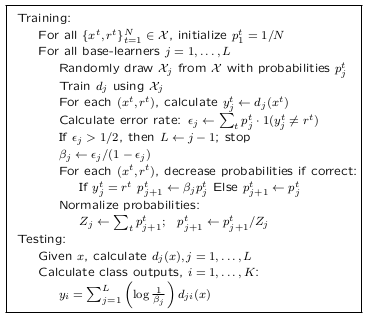
\includegraphics[width=14cm]{alg}


\end{description}
\section{Matrices Properties}
\begin{description}
    \item[Basic Matrix]
        $(\bA\bB)^T = \bB^T\bA^T$, 
    $(\bA\bB)^{-1} = \bB^{-1}\bA^{-1}$, $(\bA^T)^{-1} = (\bA^{-1})^T$, 
    $\mathbf{P}^{-1}+\bB^T \bR^{-1}\bB)^{-1}\bB^T\bR^{-1} = \mathbf{P}\bB^T(\bB
    \mathbf{P}\bB^T+\bR)^{-1}$, 
\item[Traces and Determinants] $Tr(\bA\bB) = Tr(\bB\bA)$, $Tr(\bA\bB\bC) = Tr(\bC\bB\bA) = Tr(\bB\bC\bA)$,
    $|\bA^{-1}| = \frac{1}{|\bA|}$, $\ba^T\bA\ba = Tr(\bA \ba\ba^T)$
\item[Matrix Derivatives] $\frac{\partial}{\partial \bx}(\bx^T\ba) =
    \frac{\partial}{\partial \bx}(\ba^T\bx) = \ba$,
    $\frac{\partial}{\partial\bx}(\bA\bB) = \frac{\partial \bA}{\partial \x}\bB
    +\bA\frac{\partial \bB}{\partial \bx}$, $\frac{\partial}{\partial
    x}(\bA^{-1}) = -\bA^{-1}\frac{\partial \bA}{\partial x}\bA^{-1}$, 
    $\frac{\partial}{\partial x}\ln |\bA| = Tr(\bA^{-1}\frac{\partial
    \bA}{\partial x})$, $\frac{\partial}{\partial A_{ij}}Tr(\bA\bB) = B_{ji}$,
    $\frac{\partial}{\partial \bA}Tr(\bA\bB) = \bB^T$, $\frac{\partial}{\partial
    \bA}Tr(\bA) = \mathbf{I}$, $\frac{\partial}{\partial \bA}Tr(\bA\bB\bA^T) =
    \bA(\bB+\bB^T)$, $\frac{\partial}{\partial \bA}\ln |\bA| = (\bA^{-1})^T$
\end{description}


\chapter{Convolutional Neural Networks}
\section{Motivation}
There exist a complex arrangement of cells within the visual cortex. These
cells are sensitive to small sub-regions of the input space, called a
\textbf{receptive field}, and are tiled in such a way as to cover the
entire visual field. These filters are local in input space and are thus
better suited to exploit the strong spatially local correlation present in
natural images.

Two basic cell types: Simple cells (S) and complex cells (C).
\begin{itemize}
    \item Simple Cells(S) respond maximally to specific edge-like stimulus
        patterns within their receptive field.
    \item Complex cells(C) have larger receptive fields and are locally
        invariant to the exact position of stimulus.
\end{itemize}

\section{Sparse Connectivity}
CNNs exploit spatially local correlation by \textbf{enforcing a local
connectivity pattern between neurons of adjacent layers}. 

Input hidden units in the $m$-th layer are connected to a local subset of
units in the $(m-1)$-th layer, which have spatially contiguous receptive
fields. 

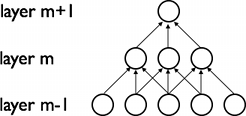
\includegraphics{sparse_1D_cnn}

\begin{itemize}
    \item Layer $m-1$ is the input retina. 
    \item Units in layer $m$ have receptive fields of width 3. Thus only
        connected to 3 adjacent neurons in the $(m-1)$-th layer.
    \item Layer $m$ have a similar connectivity with the layer below.
        $(m+1)$
\end{itemize}

We say that their receptive field with respect tot he layer below is 3,
but their receptive field with respect to the input is larger (it is 5).
The architecture thus confines the learnt ``filters'' to the spatially
local pattern.

\section{Shared Weights}
In CNNs, each sparse filter $h_i$ is additionally replicated across the
entire visual field. These ``replicated'' units form a \textbf{feature
map}, which share the same parameterization. (the receptive fields in the
same feature map share the same weight and bias for the sensitive region)

Gradient descent can still be used to learn such shared parameters, and
requires only a small change to the original algorithm. The gradient of a
shared weight is simply the sum of the gradients of the parameters being
shared.

Replicating units in this way allows for feature to be detected regardless
of their position in the visual field. Additionally, weight sharing offers
a very efficient way to do this, since it greatly reduces the number of
free parameter 

\section{Details and notation}
The $k$-th feature map at a given layer as $h^k$, whose filter with
weights $W^k$ and bias $b_k$, then the feature map $h^k$ is obtained as
follows (for $tanh$ non-linearities)
\[ h^k_{ij} = tanh\left( \left( W^k*x)_{ij} \right) + b_k \right)\]

To form a richer representation of the data, hidden layers are composed of
a set of multiple feature maps $\left\{ h^{(k)}, k = 0\dots K \right\}$

The weights of this layer can be parameterized as a 4D tensor (Tensors are
geometric objects that describe linear relations between vectors, scalars,
and other tensors. Elementary examples of such relations include the dot
product, the cross product and linear maps, vectors and scalars themselves
are also tensors.)
\begin{itemize}
    \item Destination feature map index
    \item Source feature map index
    \item Source vertical position index
    \item Source horizontal position index
\end{itemize}
\section{MaxPooling}
MaxPooling is a form of non-linear down-sampling. MaxPooling partitions
the input image into a set of non-overlapping rectangles and, for each
such sub-region, outputs the maximum value.

Useful for two reasons:
\begin{itemize}
    \item Reduces the computational complexity for upper layers
    \item Provides a form of translation invariance
\end{itemize}

Why it works: Imagine cascading a max-pooling layer with a convolutional
layer. There are $8$ directions in which one can translate the input image
into a single pixel. If max-pooling is done over a $2\times 2$ region, 
$3$ out of these $8$ possible configurations will produce exactly the same
output at the convolutional layer. For max-pooling over a $3\times 3$

\section{The Full Model: LeNet}
Graphical depiction: 

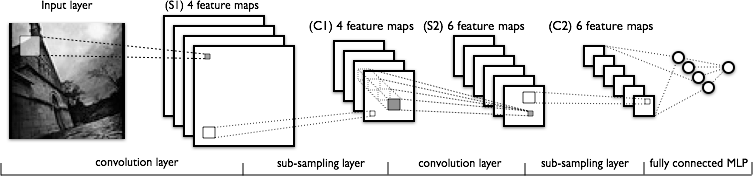
\includegraphics{mylenet}

The lower layers are composed to alternating convolution and max-mpooling
layers.

The upper layers however are fully-connected and correspond to a
traditional MLP


\chapter{Denoising Autoencoders}
An extension of a classical autoencoder and it was introduced as a
building block for deep networks. 
\section{Autoencoders}
An auto-encoder is trained to encode the input $\bx$ into some
representation $\mathbf{c}(\bx)$ so that the input can be reconstructed
from that representation. Hence the target output of the auto-encoder is
the auto-encoder input itself.

An autoencoder takes an input $ \bx\in [0,1]^d$

First maps it with an encoder to a hidden representation $\bf y \in [ 0,
1]^{d'}$ through a deterministic mapping:
\[ \by = s(\bW\bx + \mathbf{b}) \]
Where $s$ is a non-linearity such as the sigmoid. 

The latent representation $\bf y$, or \textbf{code} is then mapped back
(with a decorder ) into a \textbf{reconstruction} $\bf z$ of same shape as
$\bx$ though a similar transformation:
\[ \mathbf{z}= s(\bW' \by + \mathbf{b}')\].
Where $'$ does NOT indicate transpose, and $\mathbf{z}$ should be seen as
prediction of $\mathbf{x}$, given the code $\by$

The parameter of the model $W$ are optimized such that \textbf{the average
reconstruction error is minimized}. 

Measure the reconstruction error using the traditional squared error
$L(\bx, \mathbf{z}) = \|\bx - \mathbf{z}\|$

If the input is interpreted as either bit vectors or vectors of bit
probability by the reconstruction cross-entropy defined as (if $\bx|\by$
is in Gaussian):
\[ L_H(\bx, \mathbf{z}) = -\log P(\bx|\by) = -\sum_{k=1}^d\left[ \bx_k\log
\mathbf{z}_k + (1-\mathbf{x}_k)\log (1-\mathbf{z}_k)\right]\]

The hope: $\by$ is a distributed representation that captures the
coordinates along the main factors of variation in the data.

\section{Denoising Autoencoder}
The idea behind denoising autoencoders is that in order to force the
hidden layer to discover more robust features and prevent it from simply
learning the identity (copy the input to output), we train the autoencoder
to reconstruct the input from a corrupted version of it.

The denoising auto-encoder is a stochastic version of the auto encoder.
It does two things:
\begin{itemize}
    \item Try to encode the input (preserve the information)
    \item Try to undo the effect of a corruption process stochastically
        applied to the input of the auto-encoder.
\end{itemize}

The stochastic corruption process consists in randomly setting some of
the inputs (as many as half of them) to zero. Hence the denoising
auto-encoder is trying to \textbf{predict corrupted values from the
uncorrupted values}, for randomly selected subsets of missing patterns.
Note how being able to predict any subset of variables from the rest is a
sufficient condition for completely capturing the joint distribution
between a set of variables.

To convert the autodecoder class into a denoising autoencoder class, all
we need to do is to add a stochastic corruption step operating on the
input.



\chapter{Stacked Denoising Autoencoders(SDA)}
The denoising autoencoders can be stacked into form a deep network by
\textbf{feeding the latent representation(output code)} of the denoising
autoencoder found on the layer below as input to the current layer.

The unsupervised pre-training of such an architecture is done one layer at
a time. 

Each layer is trained as a denoising auto-encoder by minimizing
the reconstruction of its input (output code of the previous layer).

Once the first $k$-layers are trained, we can train the $(k+1)$-th layer
because we can now compute the code (latent representation) from the layer
below.

Once all layers are pre-trained, the network goes through a second stage
of training called \textbf{fine-tuning}.

\paragraph{Supervised fine-tuning} Minimize the prediction error on a
supervised task. 
\begin{enumerate}
    \item Add a logistic regression layer on top of the network (the out
        put code of the output layer)
    \item Train the entire network as we would train a multilayer
        perceptron. 
    \item At this point, we only consider the encoding parts of each
        auto-encoder.
\end{enumerate}

\chapter{Multi-Label Classification}
\section{HOMER Algorithm}
\subsection{Training}
General idea: transform large set of labels $L$ into a tree-shaped
hierarchy of simpler multi-label classification tasks.
\begin{itemize}
    \item Each node $n$ of the tree contains $L_n \subseteq L$
    \item There are $|L|$ leaves, each one containing single distinct
        label $\lambda_i \in L$
    \item Each node contains the union of the label set of its children.
        $L_{root} = L$
\end{itemize}

\emph{Meta-label}: of a node $n$, $\mu_n$ as the disjunction of the labels
contained in the node. A training example can be considered annotated with
meta-label $\mu_n$ if it is annotated with at least one of the labels in
$L_n$

Each internal node $n$ of the hierarchy also contains a multilabel
classifier $h_n$. 

Task of $h_n$: the prediction of one or more of the labels of its
children. Set of labels for $h_n$
\[
    M_n = \{ \mu_c | c \in \mbox{children}(n)\}
\]


\subsection{Prediction}
\begin{enumerate}
    \item Starts with $h_{root}$
    \item Follows a recursive process forwarding $x$ to the multilabel
        classifier $h_c$ of a child node $c$ only if $\mu_c$ is among the
        prediction of $h_{\mbox{parent}(c)}$
    \item Eventually, this process may lead to the prediction of one or
        more single-labels by the multi-label classifiers.
    \item The union of these predicted single-labels is the output of hte
        proposed approach in this case.
\end{enumerate}
\subsection{Training}
\begin{enumerate}
    \item Assume the existence of a set $D = \{(\bx_i, \bY_i) | i = 1
        \cdots |D|\}$, each one consists of a feature vector $\bx_i$ and
        set of labels $\bY_i \subseteq L$.
    \item Recursively in a top-down depth-first fashion starting with the
        root
    \item At each $n$, $k$ children nodes are first created, unless $|L_n|
        < k$, in which the number of children is $|L_n|$.
    \item Each such child $n$ filters the data of its parent, keeping only
        the eexample that are annotated with at least one of its own
        labels.
    \item Two main processes are then sequentially executed:
        \begin{enumerate}
            \item labels of the current node are distributed into $k$
                disjoint subsets, one for each child of the current node
            \item A multilabel classifier is trained for the prediction of
                the meta-labels of its children.
        \end{enumerate}
    \item The approach recurses into each child node that contains no more
        than a single label.
\end{enumerate}

Grouping: balanced k-means.

\section{RAKEL}
Let $L = \{\lambda_i\}, i = 1 \dots |L|$ be the set of labels. A set
$Y\subseteq L$ with $k = |Y|$ is called $k$-labelset.

\section{MLkNN}
\subsection{Preliminaries}
Notations
\begin{description}
    \item[domain of instances] $\mathcal{X}$
    \item[Finite set of labels] $\mathcal{Y} = \{(x_1, Y_1), (x_2, Y_2),
        \dots, (x_m, Y_m)\}, (x_i \in \mathcal{X}, Y_i \subseteq
        \mathcal{Y})$
\end{description}

Learning system will produce a real-valued function of the form:
\[ f: \mathcal{X} \times \mathcal{Y} \rightarrow \mathcal{R}\]

A successful learning system will tend to output larger values for labels
in $Y_i$ than those not in $Y_i$. That is
\[ f(x_i, y_1) > f(x_i, y_2), \forall y_1 \in Y_i, \mbox{and} y_2 \not\in
Y_i\]

The corresponding multi-label classifier $h(\cdot)$:
\[ h(x_i) = \{ y|f(x_i, y) > t(x_i), y \in \mathcal{Y}\}\]
Where $t(\cdot)$ is a threshold function which is usually set to be the
zero constant.

\subsection{ML-KNN}

Given an instance $x$ and its associated label set $Y\in \mathcal{Y}$

Let $\vec{y_x}$ be the category vector for $x$:
\[
    \vec{y_x}(l) = 
    \begin{cases}
    1 & l \in Y \\
    0 & \mbox{otherwise}
    \end{cases}
\]

Let $N(x)$ denote the set of the label sets of these neighbors, a
\emph{membership counting vector} can be defined as:

\[ \vec{C}(x) = \sum_{a \in N(x)}\vec{y_a}(l), l \in \mathcal{Y}\]

$\vec{C_x}(l)$ counts the number of neighbors of $x$ belonging to the
$l$th class.

\begin{itemize}
    \item  For each test instance $t$, ML-KNN firstly identifies its KNNs $N(t)$ in
        the training set.
    \item $N(t)$ --- neighbors of $t$
    \item $\vec{C}_t(l)$ --- membership counting vector. Number of element
        in $N(t)$ that has label $l$.
    \item $H_b^l$, $b \in {0, 1}$ --- $t$ (the testing instance) has label
        $l$ if $b = 1$, otherwise if $b = 0$
    \item $\vec{y}_x(l)$ --- $1$ if instance $x$ has label $l$
    \item $E_j^l, j \in \{0, 1, \dots, K\}$ --- Among $N(t)$ exactly $j$ instances have label $l$.
\end{itemize}

Based on the membership counting vector $\vec{C_t}$, the category vector
$\vec{y_t}$ is determined using the following MAP principle:

\[ 
    \vec{y}_t(l) = \arg\max_{b\in \{0,1 \}} P(H_b^l|E_{\vec{C}_t(l)}^l), l
    \in \mathcal{Y}
\]

Using the Bayesian rule:
\begin{align*}
    \vec{y}_t(l) &= \arg\max_{b\in \{0, 1\}} \frac{P(H_b^l)
        P(E^l_{\vec{C}_t(l)}|H_b^l)}{P(E_{\vec{C}_t(l)}^l|H_b^l)} \\
        &= \arg\max_{b \in \{0, 1\}} P(H_b^l)P(E_{\vec{C}_t(l)}^l|H_b^l)
\end{align*}

Algorithm
\begin{enumerate}
    \item For each label $l \in \cY$, calculate the prior:
        \[P(H_1^l) = \frac{(s + \sum_{i=1}^m y_{x_i}(l))}{s \times 2 +
        m}\]
        The probability that any instance has label $l$. $s$ is smoothing
        parameter. It is basically $\frac{\#\mbox{instance has
        }l}{\#\mbox{total training instances}}$.
        \[ P(H_0^l) = 1 - P(H_1^l)\]
    \item Identify the KNN $N(x_i), i \in \{1, 2, \dots, m\}$ ($m$ testing
        instances)
    \item for each label $l \in \cY$, do the following:
        \begin{enumerate}
            \item For $j \in \left\{ 0, 1,
                \dots, K \right\}$ (the possible count of labels) initialize the counting $c[j] = 0$ and
                $c'[j] = 0$
            \item For each of the training instances $i \in \left\{ 1, 2,
                \dots m \right\}$, the number of label $l$ in the
                neighbors of $x_i$:
                \[ \delta = C_{x_i}(l) \leftarrow \sum_{a\in
                N(x_i)}\vec{y}_a(l)\]

                If $\vec{y}_{x_i}(l) =  1$, that is, if instance $x_i$
                has label $l$,  then $c[\delta] \leftarrow
                c[\delta] + 1$, else $c'[\delta] \leftarrow c'[\delta]
                + 1$.

                So $c[\delta]$ is the cases that the training instance
                $x_i$ has label $l$ and among its neighbors, there are exactly
                $\delta$ instances also have label $l$, and $c'[\delta]$
                is the that $x_i$ has $\delta$ instances labeled $l$ in
                its neighbor but it is not labeled $l$.
            \item Calculate the posterior probabilities $P(E_j^l|H_b^l)$,
                probability that produce $E_j^l$ ($j$ label $l$ in
                the neighbor) given the instance $H_b^l$ (has or does not
                have label $l$)
                The probability that $l$ has $j$ instances
                \begin{equation}
                    P(E_j^l|H_1^l) = \frac{s + c[j]}{s\times{K+1} +
                    \sum_{p=0}^k c[p]}
                \end{equation}
                In words, it is (ignoring the smoothing terms):
                \[ P(\mbox{$j$ neighbors with
                label $l$}) = \frac{\#\mbox{num instances with $l$ has
                $j$ neighbors labeled $l$ neighbors}}{\#\mbox{total
                    number of $l$ instances whose
                neighbors has label $l$}} \]
                
                Similarly:
                \begin{equation}
                    P(E_j^l|H_0^l) = \frac{(s+ c'[j])}{s\times(K+1) +
                        \sum_{p=0}^k c'[p]} \end{equation}
        \end{enumerate}
\end{enumerate}

\section{Label Partition}
A data set of pairs $(x_i, y_i)$, $i = 1, \dots, m$. Possible labels
$\mathcal{D}$.

Goal: given a new example $x^*$, to rank the entire set of labels
$\mathcal{D}$ and output the top $k$ to the user which should contain the
most relevant results possible.

It is assumed that user has already trained a label scorer $f(x,y)$ that
for a given label returns a real-valued score.

Two components:
\begin{itemize}
    \item An \emph{input partitioner} that given an input example, maps it
        to one or more partitions of the input space.
    \item \emph{label assignment} which assigns a subset of labels to each
        partition.
\end{itemize}

For given example, the label scorer is applied to only the subset of
labels present in the corresponding partitions.

At prediction time:

\begin{enumerate}
    \item Given a test input $x$, the input partitioner maps $x$ to a set
        of partitions $p = g(x)$.
    \item We retrieve the label sets assigned to each partition $p_j: L =
        \cup_{j=1}^{|p|} \mathcal{L}_{p_j}, \quad p_j \in p$ where $\mathcal{L}_{p_j}
        \subseteq \mathcal{D}$ is the subset of labels assigned to
        partition $p_j$
    \item We score the labels $y \in L$ with the label scorer $f(x,y)$,
        and rank them to produce our final result.
\end{enumerate}

\subsection{Input Partitioner}
$g(x) \rightarrow p \subseteq \mathcal{P}$o
Where there are $P$ possible partitions, $\mathcal{P} = \left\{ 1, \dots P
\right\}$

Goal: to partition the input space such that examples that have the same
relevant labels highly ranked by the label scorer are in the same
partition.

For given example $(x_i, y_i)$, the accuracy:
\[\hat{l}(f(x_i), y_i)\]

The loss is to be minimized as (equivalent to max accuracy):
\begin{equation}
    l(f(x_i), y_i) = 1- \hat{l}(f(x_i), y_i)
\end{equation}

Here $f(x)$ is the vector of scores for all labels:
\[ f(x) = f_{\mathcal{D}}(x) = \left( f(x, \mathcal{D}_1), \dots,
f(x, \mathcal{D}_{|\mathcal{D}|}) \right)\]
where $\mathcal{D}_i$ is the $i$th label.

To measure the loss of partitioner:
\begin{equation}
    l(f_{g(x_i)}(x_i), y_i)
\end{equation}
Where $f_{g(x)}(x) = \left( f(x, L_1), \dots, f(x, L_{|L|}) \right)$

That is, the loss within it's partition.

Then the overall loss:
\begin{equation}
    \sum_{i=1}^m l(f_{g(x_i)}(x_i), y_i)
\end{equation}

The sum of loss of all data in their partition.

The label assignment (to partitions) $\mathcal{L}$ are unknown making the
computation above infeasible. 

The errors incurred by this model can be decomposed into components. For
given example, it receives a low or zero precision at $k$ if either

\begin{itemize}
    \item It is in a partition where the relevant labels are not in the
        set
    \item The original label scorer was doing poorly in the first place.
\end{itemize}

Guidelines:

\begin{itemize}
    \item Examples that share highly relevant labels should be mapped into
        the same partition
    \item Examples for which the label scorer performs well should be
        prioritized when learning a partitioner.
\end{itemize}

Consider the case of a partitioner that works by using the closest
assigned partition as defined by partition centroids:
$c_i$, $i = 1, \dots, P$:
\begin{equation}
    g(x) = argmin_{i=1,\dots, P}\|x - c_i\|
\end{equation}

\paragraph{Weighted Hierarchical Partitioner}
Ensuring the input partitioner prioritizes examples which already perform
well with the given label scorer is to weight each training example with
tis label scorer result:
\begin{equation}
    \sum_{i=1}^m\sum_{j=1}^P \hat{l}(f(x_i), y_i) \|x_i - c_j\|^2
\end{equation}

So if the precision of the scorer with that particular instance is high,
then the distance of that instance weights more.

The hard version, only run the $k$-means over the set of training example
with higher enough quality:
\[ \left\{ (x_i, y_i): \hat{l}(f(x_i), y_i) \geq \rho \right\} \]
We take $\rho = 1$


\end{document}
